\section{Experimental Evaluation}
In this section, an analysis of \gls{ismmdp} and \gls{immmdp} is provided.
First, we describe the settings of the experiments in \Cref{subsec:setting_exp_mtd} before presenting and discussing the results in \Cref{subsec:results_mtd}.



\subsection{Setting}
\label{subsec:setting_exp_mtd}
For all the tasks discussed in this section, we run and average the results over 10 seeds.

\subsubsection{Tasks}
\label{subsubsec:tasks_mtd}

\noindent\textbf{Pendulum for \gls{immmdp}.}\indent In this experiment, we consider the Pendulum task, already been extensively studied in this dissertation. 
We wish to empirically observe the consequences of \Cref{lem:same_distrib_psmmdp}.
Therefore, we will study the state distribution of the same policy $\pi$ trained with \gls{sac} in the undelayed \gls{mdp} and tested in a \gls{immmdp}. 
These state distributions will be compared to the state distribution of a random policy in the undelayed environment.

\noindent\textbf{Pendulum for \gls{ismmdp}.}\indent Then, we focus the experiments on the \gls{ismmdp}. 
In this first task, we explore the setting of discounted expected returns in the Pendulum environment.
We study the effect of changing the delay distribution as defined by the delay vector $\boldsymbol\lambda$ on the return of our agent. 
The policy of the agent will be learnt with A-SAC for 50.000 steps sampled from the environment. 

\noindent\textbf{Maze.}\indent As a benchmark for tests in the average reward setting, we consider a 3x3 grid world\footnote{The environment is available here:\href{https://github.com/MattChanTK/gym-maze}{link}.} where the agent must learn its way from a starting state in the upper-left corner to a goal state in the lower-right one. 
The walls present inside the grid make the task slightly more difficult. 
The agent can go in any of the four cardinal directions.
When the agent hits a wall or the limits of the environment, it remains in the same cell. 
In this environment, we compare several values of the delay vector $\boldsymbol\lambda$. 
More precisely, for $\boldsymbol\lambda=(\lambda_0,\lambda_1)$, we consider the values for $\lambda_0,\lambda_1$ in the set $\{0,0.1,\dots,0.9\}$.
The particular case $\boldsymbol\lambda=(1,0)$ is the undelayed one and $\boldsymbol\lambda=(0,1)$ corresponds to a constant 1-step delay.
since the goal is the average reward, we will consider the UCRL2 algorithm and study the regret of our agent (see \Cref{subsec:theoretical_rl}).
Note that the computation of the optimal policy even for a simple environment is more intricate in the case of \gls{ismmdp}. 
First, even if the underlying \gls{mdp} is deterministic, the initialisation of the process introduces stochasticity in the initial state.
Second, when the weights of the delay vector are not concentrated at a single element, stochasticity is further injected in the transition itself.

\subsection{Results}
\label{subsec:results_mtd}

\noindent\textbf{Pendulum for \gls{immmdp}.}\indent We report the state distributions for the three processes in \Cref{fig:state_distrib_pendulum_mtd}. 
These distributions are obtained by running several episodes of the Pendulum environment. 
Clearly, the undelayed \gls{sac} policy produces a similar state distribution on the undelayed \gls{mdp} and the \gls{psmmdp}.
This distribution is very different from that of a random policy.
One could observe an innermost parabola where only states from the undelayed process are observed.   
States with low velocity and small angle are typical in the initial steps of the process, and the fact that the delayed process does not observe such a state can be due to the delay initialisation shift (see \Cref{subsec:delay_init}). 
The first randomly sampled action from the environment gives an initial speed or angle that allows the agent to start in a different position.
This does not invalidate our theory, as these first states are transient for \gls{sac}'s close to the optimal policy. 

\begin{figure}[t]
    \centering
    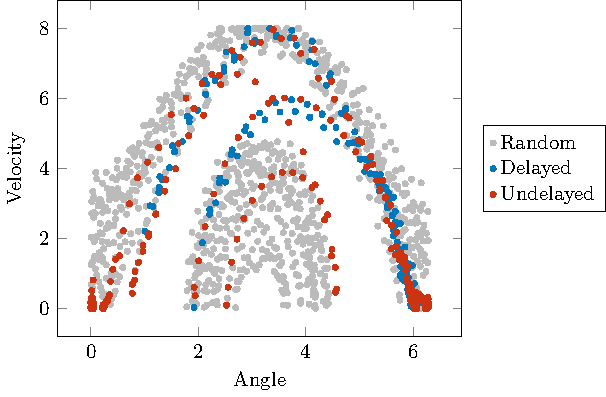
\includegraphics[labelmtdstates=statesdistribmtdpendulum]{img/thesis_plots_chapter_mtd_states.pdf}
    \caption{Comparison of the state distribution for a policy obtained with \gls{sac}, when tested in an undelayed Pendulum environment or its delayed \gls{psmmdp} counterpart. 
    The state is composed of two elements, the velocity and the angle of the pole.
    The state distribution of a random policy in the undelayed environment is added for comparison. }
    \label{fig:state_distrib_pendulum_mtd}
\end{figure}


\noindent\textbf{Pendulum for \gls{ismmdp}.}\indent The returns obtained for different values of the delay vector are shown in \Cref{fig:pendulum_mtd}. 
As the delay distribution starts to shift to longer delays, the return starts to decrease, as expected in \Cref{conj:delay_cumulativ_distrib}. 
Looking more closely at the results, it seems that when the delay vector is distributed over two consecutive values of $\lambda$, $(\lambda_i=0.5,\lambda_{i+1}=0.5)$, the performance is generally below the one of $(\lambda_{i+1}=1)$, although not significantly.
This could be against \Cref{conj:delay_cumulativ_distrib} but may only be due to a learning problem. 
In fact, the number of samples for training A-SAC is fixed for all delays, but delays of the type $(\lambda_i=0.5,\lambda_{i+1}=0.5)$ inject more stochasticity into the transition probabilities, likely making the learning of an optimal policy harder. 

\begin{figure}[t]
    \centering
    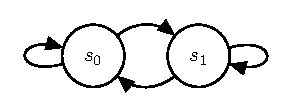
\includegraphics[labelmtd=pendulummtd]{img/thesis_plots_mtd.pdf}
    \caption{Evolution of the return for A-SAC tested on different values of the delay vector $\boldsymbol\lambda$ on the Pendulum environment. 
    Note the particular values for the undelayed ($\lambda_0=1$) and constantly $\delay$-delayed environments ($\lambda_{\delay}=1$).}
    \label{fig:pendulum_mtd}
\end{figure}

\noindent\textbf{Maze.}\indent The results are reported in \Cref{fig:grid_world_ucrl}. 
Here again, the effect of a shifting delay distribution can be observed more clearly. 
As the distribution of the delay places more weight on longer delays, the regret increases. 
Interestingly, there appears to be a gap between the constant delay cases ($\boldsymbol\lambda_0=1$ and $\boldsymbol\lambda_1=1$) and the other delay vectors.
Indeed, although arranged by cumulative distribution, the regrets for stochastic delays are clustered and significantly away from constant delays regrets.

\begin{figure}[t]
    \centering
    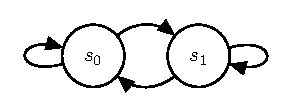
\includegraphics[labelmtd=gridworld]{img/thesis_plots_mtd.pdf}
    \caption{
    Evolution of the regret for UCRL2 tested on different values of the delay vector $\boldsymbol\lambda$ on the Maze environment. 
    Note the particular cases of the undelayed ($\boldsymbol\lambda=(1,0)$) and constant 1-step delayed ($\boldsymbol\lambda=(0,1)$) processes.}
    \label{fig:grid_world_ucrl}
\end{figure}
